\documentclass[runningheads]{llncs}
%\documentclass{sig-alternate}
\usepackage{bussproofs}
\usepackage{amssymb}
\usepackage{graphicx}
\usepackage{url}
\usepackage{color}
\usepackage{proof}
\usepackage{qtree}
\newcommand\tool[1]{\textsf{#1}}
\newcommand\vmdv{\tool{VMDV}}
\newcommand\couic[1]{}

%
\begin{document}
	
\title{\vmdv: A 3D Visualization Tool for Modeling, Demonstration, and Verification}

\couic{\author{
       \IEEEauthorblockN{Jian Liu\IEEEauthorrefmark{1}\IEEEauthorrefmark{2},
       Ying Jiang\IEEEauthorrefmark{1} and
       Yanyun Chen\IEEEauthorrefmark{1}}
}}

\author{}


\maketitle

\begin{abstract}
In the setting of automated theorem proving,
the output of an automated theorem prover is usually presented in text format,
which is often too heavy to be understood. 
In the setting of model checking, 
it would be helpful if one can observe, at the same time, 
both the model structure under consideration and the verification procedure. 
To address these problems, 
a 3D visualization tool for modeling, demonstration and verification (\vmdv{} for short) is proposed in this paper. 
The facilities of \vmdv{} are illustrated by applying it to an automated theorem prover.

\keywords{3D Visualization \and Automated theorem proving \and Model Checking} 

\end{abstract}

\section{Introduction}
In the field of mathematical logic, a formal proof is usually defined as a sequence of formulas,
which are either axioms or logical consequences of the preceding formulas. 
In the most natural way, a proof is generally presented as a proof tree, where
each node is labeled by a formula, and its children are labeled by its hypothesis. 
Nowadays, one can obtain proofs from computers automatically,
thanks to the development of automated theorem provers. 
However, the output of a theorem prover is usually displayed in text format. 
This usually makes the proof tree difficult to understand 
(e.g., to observe the relative locations of some nodes in the same proof tree), 
especially when the proof tree contains a large set of nodes. 
The same problem also arises in the field of model checking, 
where counterexamples generated by model checkers are sometimes hard to read \cite{CBJPK,CGP01,CGMZ}. 
Moreover, text format is difficult to show the proof structures, when proof trees are dynamically updated. 
This is very common in a proving procedure, where the nodes may be dynamically created or deleted.
Thus, 
a more readable form will be helpful to engineers who are not familiar with model checking or automated theorem proving. 
This leads to the following questions which motivate the present work: 

\begin{enumerate}
\item 
How to make the output of a theorem prover to carry huge amount of information and, at the same time,  easy to understand and to reason about?
\item 
How to observe the verification procedure in an intuitive manner when checking some properties of a given complex model?
\end{enumerate}

To answer these questions, 
a 3D visualization tool for Modeling, Demonstration, and Verification (\vmdv{} for short) is proposed\footnote{\url{https://github.com/terminatorlxj/VMDV}}.
\vmdv{} represents proofs by 3D trees.
As a matter of fact, 
\vmdv{} employs a 3D renderer to plot proof trees in 3D space. 
As is well known, 3D renderer is based on the 3D information visualization techniques
which take advantage of the human eyes' broad bandwidth pathway into the mind to allow users to capture large amounts of information at once.
In this way, proof trees are easily organized and displayed,
detailed local text information adheres to the node on demand.

In Fig. \ref{fig:compare_text_graph_detail},
it is shown that the 2D format is more convenient to reflect the structure of the proof tree than the text format.
However, when a proof tree contains a large number of nodes, 
the information adhering to the nodes may be overlapped, and hence hard to understand, even to read.
In contrast, there is enough space in 3D format to show, without confusion, both the structure of proof trees and the information adhering to the nodes. 
One of the reasons is that a 3D format space can be seen as a combination of infinitely many 2D plans, and \vmdv{} allows to
observe an output of an automated theorem prover, typically a proof tree, from different angles by rotating and zooming.

\begin{figure}[!h]
\centering
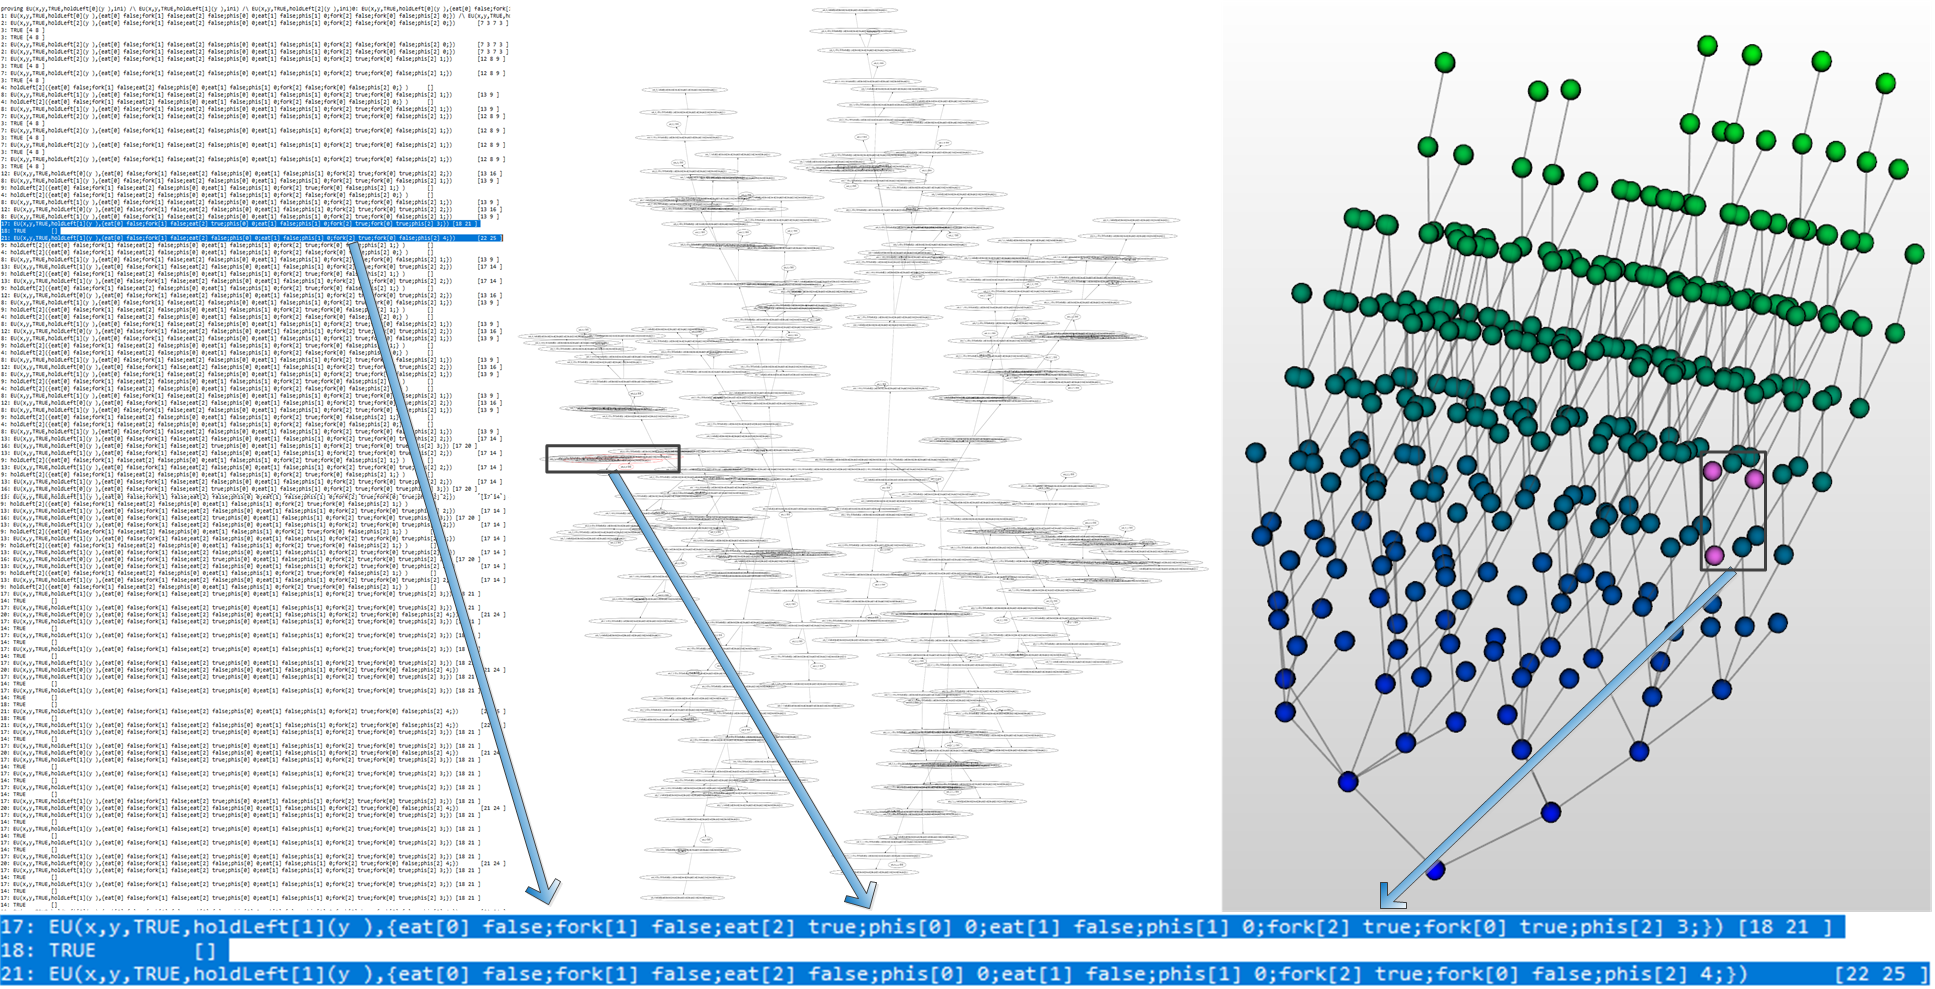
\includegraphics[width=9cm]{./compare_123.png}
\caption{Display of a proof tree in text format, 2D format, and 3D format, respectively.} 
\label{fig:compare_text_graph_detail}
\end{figure}

The main facilities of \vmdv{} are listed as follows.
They are illustrated by applying \vmdv{} to \textsf{SCTLProV}\footnote{https://github.com/terminatorlxj/SCTLProV},
which can be seen both as an automated theorem prover and a model checker.

\begin{itemize}
\item
\vmdv{} allows the observation either from a global view or from a local view. 
The global view shows the shape, or the topological structure of the concerned output,
while the local view shows the detailed information of nodes or sub-structures under consideration
(Fig. \ref{fig:screenshot}). 

\item
\vmdv{} also provides us a variety of ways to observe or interact with the proof tree. 
The zooming and rotation operations effectively change the viewport, making the presentation of the overall structure of the proof tree clear via different angles of view (Fig. \ref{fig:prooftree_angles}).

\item
When the output, typically a proof tree, is very large and only a subtree is of interest, 
this subtree can be selected and focused, while other parts of the tree can be hidden; 
also, nodes with specific pattern can be searched and highlighted on the proof tree etc. (Fig. \ref{fig:high_different}). 
This allows us to find, among others, all the formulas from which one specific formula can be inferred or deduced.
\couic{
The same scenario holds in the setting of model checking (Fig. \ref{fig:state_angles}).
}
 
\item
In some proof systems, there may be some auxiliary structures emerging along with the construction of proof trees, 
such as Kripke models or inductively defined terms. 
\vmdv{} visualizes both proof trees and auxiliary structures.
Visualizing the interaction between proof trees and the auxiliary structures may help us to better understand the proving procedure.
\end{itemize}

As a visualization tool, \vmdv{} is designed and implemented as a stand-alone program, 
which is independent of the automated theorem prover to be applied.
Indeed, automated theorem provers and \vmdv{} communicate via TCP sockets (Fig. \ref{fig:architecture}). 
This facilitates the extensibility of \vmdv{} to different automated theorem provers. 
%Design such a visualization interface for existing proof systems such as Coq is our future work. 
\smallskip

\hspace{-0.5cm}
{\bf \it Related Work.} 
As far as we know, many efforts have been made to the visualization of the output of automated theorem provers. 
For instance, in \cite{byrnes2009visualizing,LibalRR14,sakurai2011mikibeta}, and \cite{steel2005visualising}, 
proofs are presented in 2D format instead of text format, and colors are used to highlight crucial parts of proof trees.
In \cite{LibalRR14}, the authors proposed several criteria for the visualization of proof trees, 
such as distinguishing different kinds of rules, 
following the progress of subproofs, and focusing on different aspects of the proof, etc.
On the other hand, there exist indeed a few visualization tools with 3D libraries (\cite{Farmer200939,bajaj2003interactive}), 
and with the facility for visualizing both proof trees and other data structures such as term expressions \cite{bajaj2003interactive},
however the layout algorithms of these tools are only limited to graphs with simple structures. 
Our work is different from the existing visualization tools:
First, we render the graphs in 3D format, instead of 2D format as in most of the existing visualization tools.
Rendering in 3D space enables the visualization of graphs with much more complicated structures that are usually difficult to understand in 2D space. 
Secondly, we use an automatic layout algorithm which simulates a physical system where nodes repulse each other like magnets, while edges attract the nodes that they connect like springs. 
This algorithm is capable of handling the layout of the proof tree smoothly, where nodes may be hidden, created, or deleted dynamically during a proving procedure.
\smallskip

\hspace{-0.5cm}
{\it Outline.} 
The rest of the paper is organized as follows: 
Section \textsf{II} presents the preliminaries, 
including some basic notions of information visualization, and the brief introduction of a proof system, called \textsf{SCTL}.  
Section \textsf{III} introduces our visualization tool \textsf{VMDV}. 
Section \textsf{IV} involves the applications of \vmdv{} to the prover of \textsf{SCTL}. 
Section \textsf{V} concerns conclusion and future works.

\section{Preliminaries}
In this section, we first present the concept of information visualization, and then present the basic definitions of a proof system called \textsf{SCTL} which is a sequent calculus for Computation Tree Logic (\textsf{CTL}) \cite{EmersonC82,EmersonH85}, and also an automated theorem prover \textsf{SCTLProV} that implements the \textsf{SCTL} system.

\subsection{Information Visualization}
Information visualization is the study of visual representation of abstract data that focus on the creation of approaches for humans to capture abstract information intuitively. With the visual representations of data, it is easier for humans to get a deeper understanding, and gain the essentials over the massive data-sets.
 
Benefit from the study of computer graphics, information presentation using visualization has been enjoying popular support.  The Open Graphics Library (\textsf{OpenGL}) provides a language independent and cross-platform application programming interface (\textsf{API}) for the rendering of three dimensional graphics. As for the hardware, the enhancing of the computational power of Graphics Processing Units (\textsf{GPU}) has made the efficient rendering of complex graphics a reality. As opposed to digital numbers which are more readable for computers, Visualization systems are more friendly to human beings for providing both concrete and abstract inspirations. For instance, plotted charts are better understandable than bare data-sets. It assists in uncovering the trends, reveal insights, or even tell stories. Information visualization provides a easier way for users to capture the abstract patterns of the massive data by applying a graphical presentation.
 
We applied the ideas of information visualization to the development of \textsf{VMDV}, as it provides:
\begin{itemize}
       \item The presentation of data in 3D space, where the data points are encoded as 3D solid spheres, and the structure of data are encodes as lines between solid spheres;
       \item Visual interaction with data, such as highlighting the search results for specific data, or controlling the progress of producing new data.
\end{itemize}
 
\subsection{\textsf{SCTL} and \textsf{SCTLProV}}
Model checking \cite{CGP01,EmersonC82,EmersonH85} and automated theorem proving
\cite{Fitting96,Loveland78} are two major pillars of formal verification methods.
The proof system \textsf{SCTL}, introduced in \cite{dowek2013logical}, is a sequent calculus for \textsf{CTL},
taking Kripke models as parameters.
\textsf{SCTL} performs verification directly on a given Kripke model from the perspective of automated theorem proving,
and produces formal proofs when the verification procedure terminates.
 
The syntax of \textsf{SCTL} is stipulated as follows.
The properties of a Kripke model are expressed in a language tailored for this model.
The language contains,
for each state $s$ of the model, a constant also written $s$; 
for each relation $P$ over the model, a predicate symbol also written $P$.
Formulas are built in the usual way with the connectors $\top$, $\bot$, $\wedge$, $\vee$ and $\neg$, to which we add modalities $AX$, $EX$, $AF$, $EG$, $AR$, and $EU$. If $\phi$ is a formula, and $t$ is either a constant or a variable, then $AX_x(\phi)(t)$, $EX_x(\phi)(t)$, $AF_x(\phi)(t)$, and $EG_x(\phi)(t)$ are formulas. Like quantifiers, modalities bind the variable $x$ in $\phi$. If $\phi_1$ and $\phi_2$ are formulas and $t$ is either a constant or a variable, then $AR_{x,y}(\phi_1,\phi_2)(t)$ and $EU_{x,y}(\phi_1,\phi_2)(t)$ are formulas. These modalities bind the variable $x$ in $\phi_1$ and $y$ in $\phi_2$, respectively.
 
The semantics of a \textsf{SCTL} formula is defined as follows, 
the proof rules for the system \textsf{SCTL} is depicted in Fig. \ref{fig:sctl_rules}.
 
\begin{definition}[Valid formula]
Let $\mathcal{M}$ be a model and $\phi$ be a closed formula, the set of valid formulas $\models \phi$ in the model $\mathcal{M}$ is defined by induction on $\phi$:
 
\begin{itemize}
        \item $\models P(s_1,...,s_n)$, if $\langle s_1,...,s_n\rangle \in P$; \  \  \  $\models \neg P(s_1,...,s_n)$, if $\langle s_1,...,s_n\rangle \notin P$,
        \item $\models \top$, \  \   \  $\models \bot$ is never the case;
        \item $\models \phi_1\wedge\phi_2$, if $\models \phi_1$ and $\models \phi_2$,
        \item $\models \phi_1\vee\phi_2$, if $\models \phi_1$ or $\models \phi_2$,
        \item $\models AX_x(\phi_1)(s)$, if for each state $s'$ in $Next(s)$, $\models (s'/x)\phi_1$,
        \item $\models EX_x(\phi_1)(s)$, if there exists a state $s'$ in $Next(s)$ such that $\models (s'/x)\phi_1$,
        \item $\models AF_x(\phi_1)(s)$, if for all infinite paths $s_0,s_1,...$ starting from $s$, there exists a natural number $i$, such that $\models (s_i/x)\phi_1$,
        \item $\models EG_x(\phi_1)(s)$, if there exists an infinite path $s_0,s_1,...$ starting from $s$, such that for all natural numbers $i$, $\models (s_i/x)\phi_1$,
        \item $\models AR_{x, y}(\phi_1,\phi_2)(s)$, if for all infinite paths $s_0,s_1,...$ starting from $s$, and for all $j$, either $\models (s_j/y)\phi_2$ or there exists an $i<j$ such that $\models (s_i/x)\phi_1$,
        \item $\models EU_{x, y}(\phi_1,\phi_2)(s)$ if there exists an infinite path $s_0,s_1,...$ starting from $s$ and a natural number $j$ such that $\models (s_j/y)\phi_2$ and for all $i<j$, $\models (s_i/x)\phi_1$.
\end{itemize}
\end{definition}
 
An automated theorem prover \textsf{SCTLProV} is developed to implement \textsf{SCTL}.
The interested reader is referred to \cite{dowek2013logical} and \cite{LiuDJJ16} for further details of the proof system \textsf{SCTL} and the automated theorem prover \textsf{SCTLProV}.
 
 
\begin{figure}[t]
\noindent\framebox{\parbox{.98\textwidth}{\hspace*{-0.3cm}
$$\scriptsize
\begin{array}{@{}lll@{}}
\infer[^{\mbox{atom-\textsf{R}}}_{\langle s_1,...,s_n\rangle \in P}]{\vdash P(s_1,...,s_n)}{}
&
\hspace{5mm} \infer[^{\mbox{$\neg$-\textsf{R}}}_{\langle s_1,...,s_n\rangle \notin P}]{\vdash \neg P(s_1,...,s_n)}{}
&
\hspace{5mm} \infer[^{\mbox{$\top$-\textsf{R}}}]{\vdash \top}{}
 
\vspace{2mm}\\
 
\infer[^{\mbox{$\wedge$-\textsf{R}}}]{\vdash \phi_1\wedge\phi_2}{\vdash \phi_1 & \vdash \phi_2}
&
\hspace{5mm} \infer[^{\mbox{$\vee$-{$\mathsf{R_1}$}}}]{\vdash \phi_1\vee\phi_2}{\vdash \phi_1}
&
\hspace{5mm} \infer[^{\mbox{$\vee$-{$\mathsf{R_2}$}}}]{\vdash \phi_1\vee\phi_2}{\vdash \phi_2}
\vspace{2mm}\\
 
\infer[^{\mbox{$\mathbf{EX}$-\textsf{R}}}_{s'\in \textsf{Next}(s)}]{\vdash EX_x(\phi)(s)}{\vdash (s'/x)\phi}
&
\multicolumn{2}{l}{\hspace{5mm}
\infer[^{\mbox{$\mathbf{AX}$-\textsf{R}}}_{\{s_1,...,s_n\}=\textsf{Next}(s)}]{\vdash AX_x(\phi)(s)}{\vdash (s_1/x)\phi & \ldots & \vdash (s_n/x)\phi}
}
\vspace{2mm}\\
 
\infer[^{\mbox{$\mathbf{AF}$-{$\mathsf{R_1}$}}}]{\Gamma \vdash AF_x(\phi)(s)}{\vdash (s/x)\phi}
&
\multicolumn{2}{l}{\hspace{5mm}
\infer[^{\mbox{$\mathbf{AF}$-{$\mathsf{R_2}$}}}_{\{s_1,...,s_n\}=\textsf{Next}(s)}]{\Gamma \vdash AF_x(\phi)(s)}{\Gamma\vdash AF_x(\phi)(s_1) & \ldots & \Gamma\vdash AF_x(\phi)(s_n)}
}
\vspace{2mm}\\
 
\multicolumn{2}{l}{
  \infer[^{\mbox{$\mathbf{EG}$-\textsf{R}}}_{s' \in \textsf{Next}(s)}]{\Gamma \vdash EG_x(\phi)(s)}{\vdash (s/x)\phi & \Gamma,EG_x(\phi)(s)\vdash EG_x(\phi)(s')}
}
&
\infer[^{\mbox{$\mathbf{EG}$-\textsf{merge}}}_{EG_x(\phi)(s)\in \Gamma}]{\Gamma \vdash EG_x(\phi)(s)}{}
\vspace{2mm}\\
 
\multicolumn{3}{c}{
  \infer[^{\mbox{$\mathbf{AR}$-{$\mathsf{R_1}$}}}_{
{
\begin{tabular}{@{}l}
{\tiny $\{s_1,...,s_n\}=\textsf{Next}(s)$}\\
{\tiny $\Gamma' = \Gamma,AR_{x,y}(\phi_1,\phi_2)(s)$}
\end{tabular}
}
}
]{\Gamma \vdash AR_{x,y}(\phi_1,\phi_2)(s)}{\vdash (s/y)\phi_2 & \Gamma'\vdash AR_{x, y}(\phi_1,\phi_2)(s_1) ~...~ \Gamma'\vdash AR_{x, y}(\phi_1,\phi_2)(s_n)}
}
\vspace{2mm}\\
 
\multicolumn{3}{l}{
\infer[^{\mbox{$\mathbf{AR}$-{$\mathsf{R_2}$}}}]{\Gamma \vdash AR_{x,y}(\phi_1,\phi_2)(s)}{\vdash (s/x)\phi_1 & \vdash (s/y)\phi_2}
~~~~~~~~
\infer[^{\mbox{$\mathbf{AR}$-\textsf{merge}}}_{AR_{x,y}(\phi_1,\phi_2)(s)\in \Gamma}]{\Gamma \vdash AR_{x,y}(\phi_1,\phi_2)(s)}{}
}
\vspace{2mm}\\
 
\multicolumn{3}{l}{
  \infer[^{\mbox{$\mathbf{EU}$-{$\mathsf{R_1}$}}}]{\Gamma\vdash EU_{x,y}(\phi_1,\phi_2)(s)}{\vdash (s/y)\phi_2}
~~~~~~~
  \infer[^{\mbox{$\mathbf{EU}$-{$\mathsf{R_2}$}}}_{s'\in \textsf{Next}(s)}]{\Gamma\vdash EU_{x,y}(\phi_1,\phi_2)(s)}{\vdash (s/x)\phi_1 & \Gamma\vdash EU_{x,y}(\phi_1,\phi_2)(s')}
  }
\end{array}
$$
 
}}
%\vspace{-10pt}
\caption{\textsf{SCTL}$({\cal M})$}
\label{fig:sctl_rules}
\end{figure}
%\vspace{-20pt}

\section{\vmdv{}}
% \vspace{-5pt}
\subsection{Architecture}
% \vspace{-5pt}
 
% \vspace{-10pt}
\begin{figure}[!h]
\scriptsize
%\vspace{2.5cm}
\centering
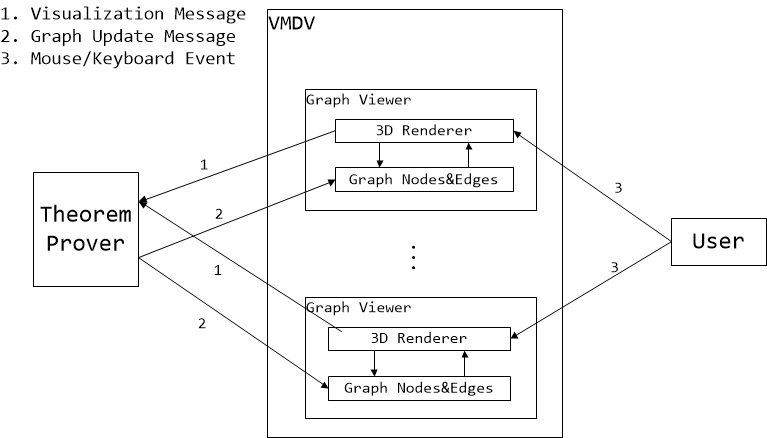
\includegraphics[width=9cm]{./architecture.png}
\caption{The architecture of \textsf{VMDV}.}
%\vspace{-10pt}
\label{fig:architecture}
\end{figure}
In the design of \vmdv{}, the theorem prover is not supposed to know exactly how \vmdv{} renders graphs, and \vmdv{} does not know the working procedure of the theorem prover. The theorem prover simply sends output information to \textsf{VMDV}, and receives feedbacks from it. As is shown in Fig. \ref{fig:architecture}, there are two kinds of messages interchanged by a theorem prover and \vmdv{}: the Visualization Messages sent by \vmdv{}, and the Graph Update Messages sent by the theorem prover. Visualization Messages are control messages consist of requiring the related information of the current formula, such as the hypothesis, sub-formulas, or other specific information (e.g., the related state in an SCTL formula). Graph Update Messages are data messages consist of the responds to the control messages.
\vmdv{} serves as the interface to dynamically visualize the output of the theorem prover. The relationship of \vmdv{} and a theorem prover is very similar to that of a web browser and a web server. In order to extend the applications of \vmdv{} to other theorem provers, \vmdv{} is designed and implemented as a stand-alone program, not as a part of specific theorem provers. Theorem provers and \vmdv{} communicate via TCP sockets. Both control and data messages are wrapped as TCP packets.  This way, \vmdv{} can easily communicate with theorem provers implemented in different programming languages, or run in different computers in networks.
 
Note that \vmdv{} allows multiple outputs to visualize multiple structures, proof trees, or, e.g., proof trees and Kripke models in \textsf{SCTL} system.
 
\vmdv{} is implemented in Java\footnote{\url{https://www.oracle.com/java/index.html}} and rendered using \textsf{JOGL},\footnote{\url{http://jogamp.org/jogl/www/}} the Java binding of the \textsf{OpenGL} \textsf{API}.
 
%\vspace{-10pt}
\subsection{Interfaces}
%\vspace{-5pt}
Fig. \ref{fig:screenshot} shows a typical screenshot of \textsf{VMDV}. It consists of two panels: the main panel on the top shows the overall structure of the proof tree, and the panel at the bottom shows the details of the selected nodes.
Similar to other 3D visualization tools, \vmdv{} adopts some commonly used operations (for instance, zooming, rotation, and selection) to interact with 3D graphs. Furthermore, \vmdv{} provides mechanisms to extend its functionalities to fulfill the special requirements of different kinds of theorem provers.
\begin{figure}[h]
\centering
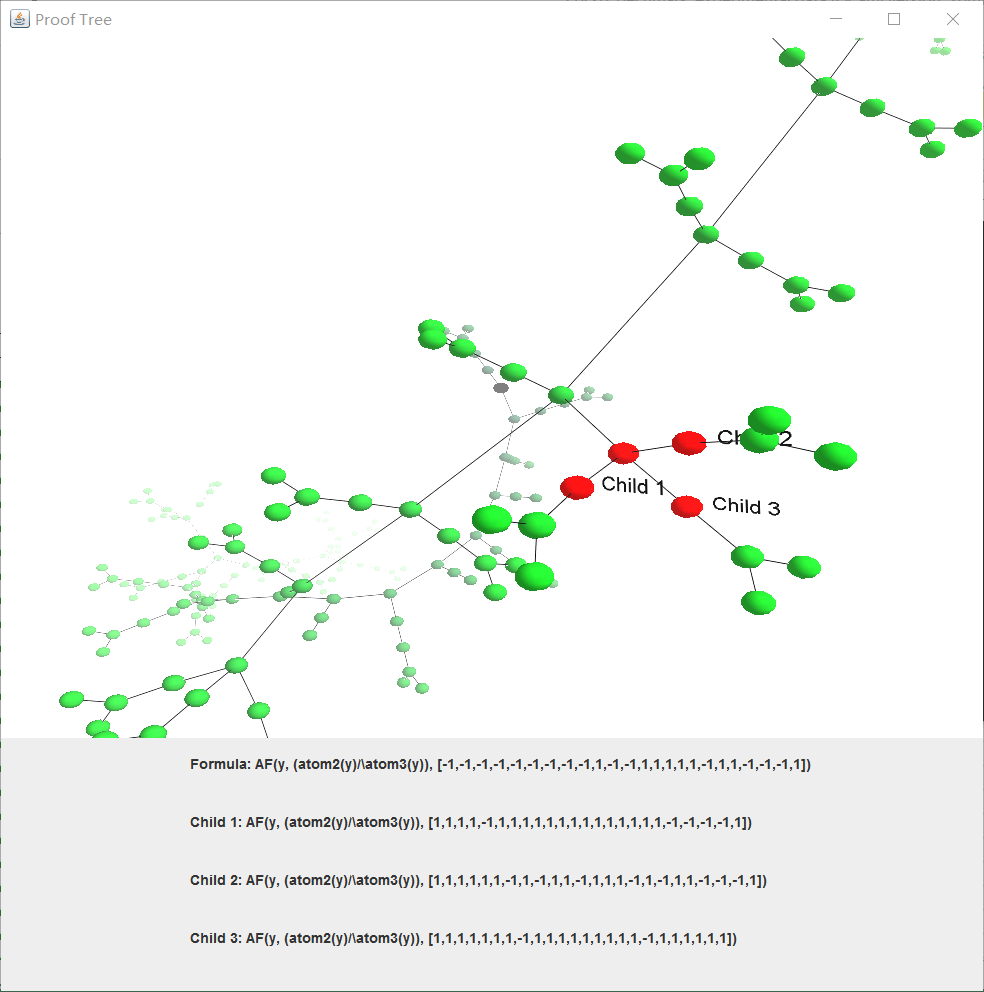
\includegraphics[width=6.5cm]{./050407.png}
%\caption{Screenshots of VMDV: the left picture consists a local panel showing children of a selected node, while the right picture consists a local panel showing ancestors of a selected node.}
\caption{A typical screenshot of \textsf{VMDV}.}
\label{fig:screenshot}
\end{figure}
\smallskip

\hspace{-0.5cm}
{\bf Zooming and rotation.}
The most obvious advantage of 3D visualization over 2D one is the capacity of observing a graph from different angles of view. Although there exist different ways to plot a 2D graph, it is still hard to match the 3D solution when the structure of the graph is too complicated to present in 2D space. 3D visualization techniques handle this easily using two operations, zooming and rotation: zooming in to see the details, zooming out to capture the overall shape, and rotating the tree to locate the sub-tree of interest, as are shown in Fig. \ref{fig:prooftree_angles}.
 
\begin{figure}[h]
\centering
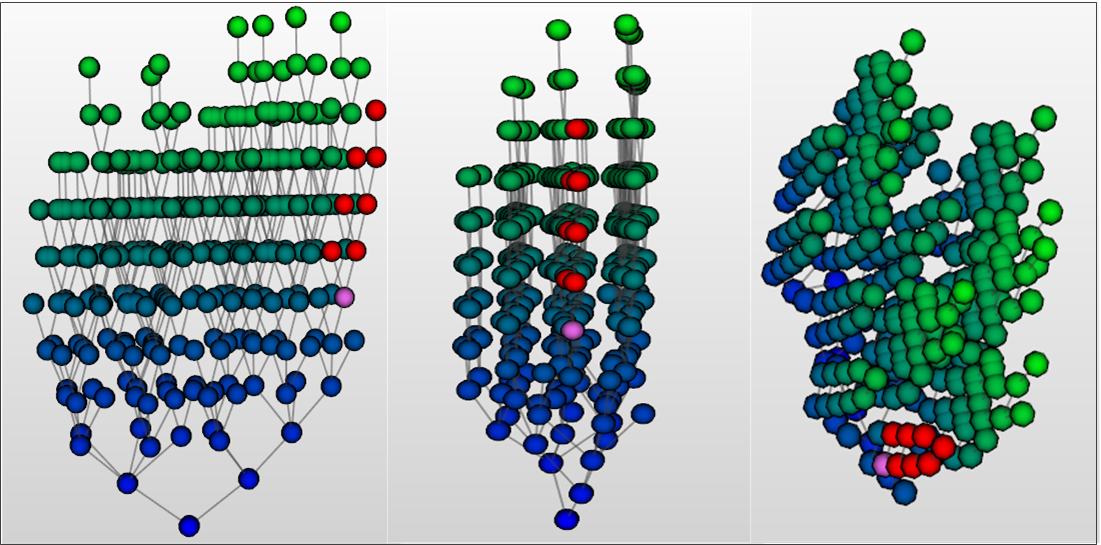
\includegraphics[width=9cm]{./phi_prooftreegraph_angles.png}
\caption{A proof tree observed from different angles of view.}
%\vspace{-10pt}
\label{fig:prooftree_angles}
%\vspace{0.8cm}
\end{figure}
%\vspace{-0.5cm}
 
 
\begin{figure}[h!]
\centering
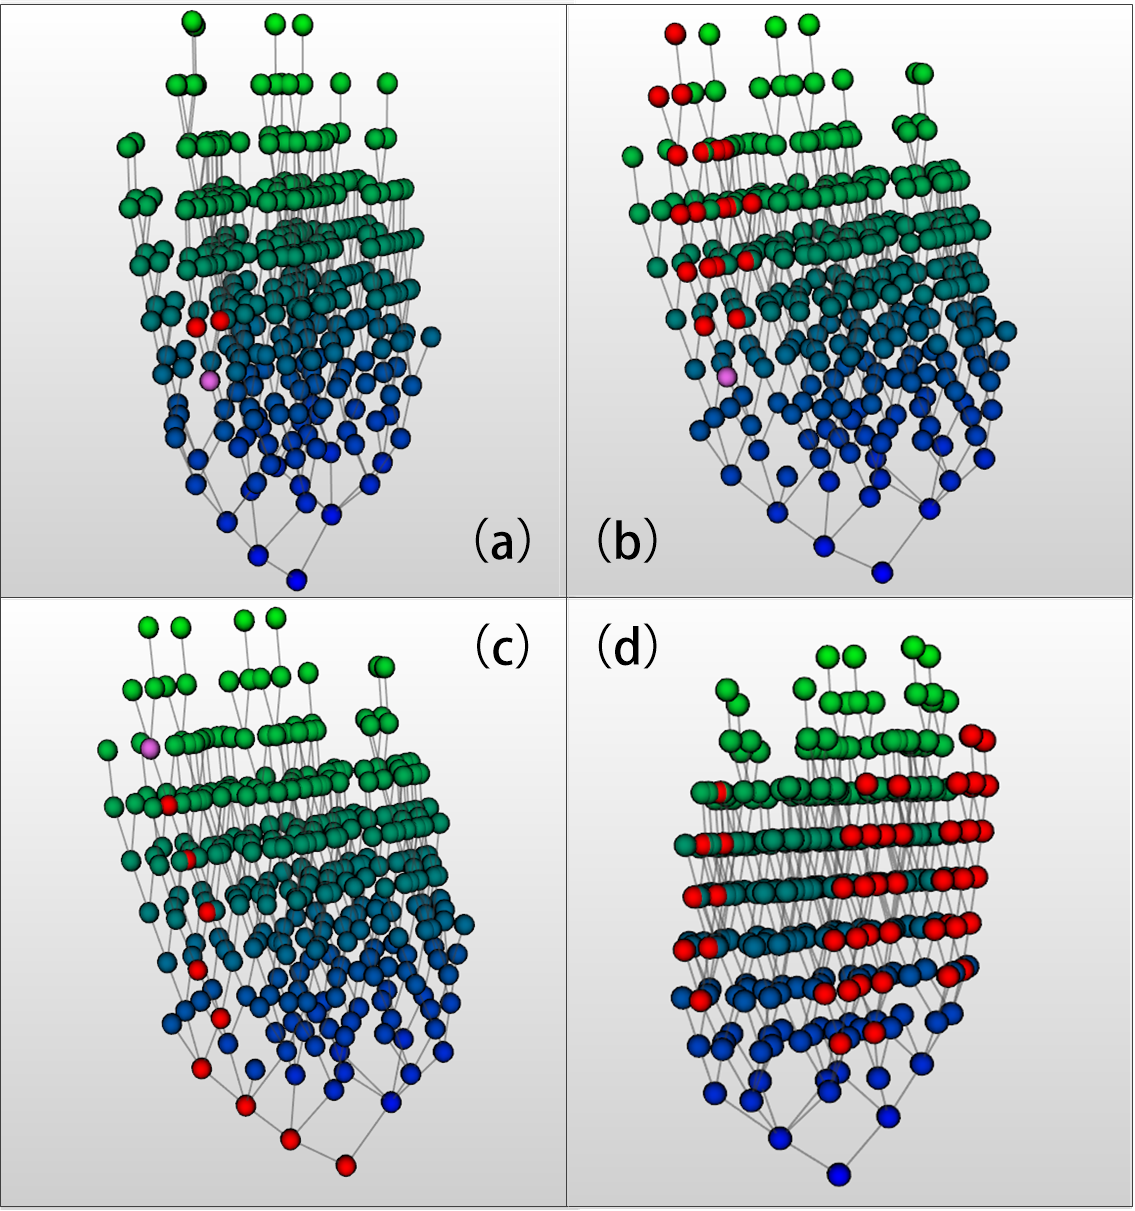
\includegraphics[width=9cm]{./high_different.png}
\caption{Different kinds of highlighting: (a) selection of a single node and its children; (b) selection of a subtree; (c) highlighting ancestors of a node; (d) highlighting similar proof patterns.}
\label{fig:high_different}
\end{figure}
\begin{figure}[h!]
\centering
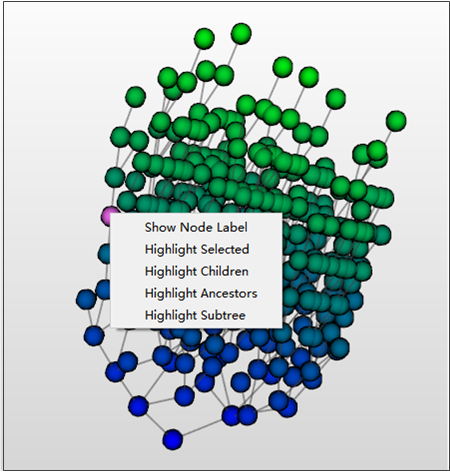
\includegraphics[width=9cm]{./user_defined_operation.png}
\caption{Extensible operations.}
%\vspace{-10pt}
\label{fig:user_defined_operation}
\end{figure}
\smallskip

\hspace{-0.48cm}
{\bf Highlighting.}
Sometimes some local information (for instance, specific nodes, edges, or proof patterns) is more interesting rather than the overall structure. Highlighting becomes a useful operation to show the local focused parts of the given proof tree. \vmdv{} enables highlighting parts of the proof tree either by manual selection using mouse clicking, or by automatic selection via formulae searching. (Fig. \ref{fig:high_different})\footnote{In \vmdv{}, we say that the proofs of two formulas have similar pattern if the first rules applied in the two bottom-up proofs are the same. For instance, if the proofs of two formulas in \textsf{SCTL} have similar pattern, then according to the rules in Fig. \ref{fig:sctl_rules}, both formulas must have the same modality or connector, or both are atomic formulas with the same predicate.}
\smallskip

\hspace{-0.5cm}
{\bf Focusing on a specific subtree.}
In many cases, interesting information may be carried out by specific subtrees. To concentrate on these subtrees, the nodes that are not related are hidden. Additional operations can then be applied only on these subtrees. The focusing of a subtree is easily done by changing the root node. A reset operation will recover the entire tree (Fig. \ref{fig:prooftree_angles}).
 
 
\vspace{0.1cm}
\hspace{-0.5cm}
{\bf Extended Operations.}
In addition to the commonly used operations, some other operations that are specific to theorem provers are also needed, so that \vmdv{} can be adapted to different theorem provers. The controlling of the construction of both the proof tree and the Kripke model in the \textsf{SCTL} system is a good example. The defining of a new operation in \vmdv{} includes two steps: first, define a set of actions that can be applied to 3D graphs; second, define triggers to activate these actions. In the first step, we wrap actions that can be applied to 3D graphs as \textsf{Affect} objects that all implement a Java interface named \textsf{AssistAffect}. Thus, new actions can be defined by adding new \textsf{Affect} objects that implement \textsf{AssistAffect}. In the second step, we define a set of \textsf{Trigger} objects that can be used to trigger the newly defined actions in the first step. All \textsf{Trigger} objects implement an Java interface \textsf{PopupItem}, which can be added to \vmdv{} as pop-up menu items at the initialization phrase of the GUI. One can select a pop-up menu item to activate a \textsf{Trigger} object when right clicked the mouse. (Fig.~\ref{fig:user_defined_operation})
 
This way, defining operations for new theorem provers in \vmdv{} can be implemented by defining new \textsf{Affect} objects and \textsf{Trigger} objects. \vmdv{} exposes simple, but powerful interfaces to the definitions of both \textsf{Affect} and \textsf{Trigger} objects.
 
 
%\vspace{-10pt}
\subsection{Automatic Layout}
%\vspace{-5pt}
The layout of 3D graphs is non-trivial. Our solution is modified from ForceAtlas2 \cite{jacomy2014forceatlas2}. ForceAtlas2 is a force-directed algorithm that simulates a physical system, where nodes repulse each other like magnets while edges attract the nodes they connect like springs. The forces of repulsion and attraction make the movement of nodes until all nodes in the 3D graph reach a balanced state. Since the clustering of nodes are not the main concern of \textsf{VMDV}, we set the degree of each node to be constant $1$ in our algorithm, not the number of edges that are attached to the node as ForceAtlas2 does. As the same as ForceAtlas2, our algorithm is continuous and homogeneous, as opposed to the OpenOrd \cite{martin2011openord} algorithm which is not, and the algorithm of Yifan Hu \cite{yifanhu05} which is semi-continuous. The continuity and homogeneity of the algorithm make the movement of nodes to respect the feeling of a physical system, and users comprehend the 3D graph by ``playing" with it.
 

\section{Applications}
%In this section, we applies \vmdv{} to \textsf{SCTL} and alternating pushdown systems.
%\vspace{-5pt}
In this section, we first show how \vmdv{} can visualize output from \textsf{SCTLProV}, and then illustrate how \vmdv{} visualize proof trees produced by the existing theorem prover Coq \cite{bertot2013interactive}.
 
%\vspace{-10pt}
\subsection{\textsf{SCTLProV}}
%\vspace{-5pt}
With the application of \textsf{VMDV}, we can show both proof trees and Kripke models in 3D format.
We can also visualize, in 3D format, the verification procedure,
revealing gradually the relation between a proof tree and the corresponding states of the Kripke model under consideration.
Although the Kripke model in realistic cases may be very large, thanks to the on-the-fly style of proof search in \textsf{SCTLProV}, we can only show the states that are necessary to be explored, which may be a small part of the whole model.
The application of \vmdv{} to the theorem prover \textsf{SCTLProV} is illustrated in the following small example.
 
\begin{example}[The River Crossing Puzzle.]
\label{expl:river}
A farmer is trying to transport a wolf, a goat, and a cabbage from one side of a river to another, however, he can only carry at most one item each time. During the transportation, the goat cannot be left alone with the wolf, nor the cabbage can be left alone with the goat.
The question is how can the farmer get across the river by bringing the wolf, the goat, and the cabbage.
\end{example}
 
We formalize this problem by defining a Kripke model,
where each state is represented by an assignment of four boolean state variables \textsf{farmer}, \textsf{wolf}, \textsf{goat} and \textsf{cabbage}, and
each transition between states is represented by the transformation of an assignment of these variables to another.
The property to be verified is that whether there is a path that starts with the state
\begin{center}
$\mathsf{S_0}$: \textsf{\{farmer:false, wolf:false, goat:false, cabbage:false\}}
\end{center}
and end with the state
\begin{center}
$\mathsf{S}$: \textsf{\{farmer:true, wolf:true, goat:true, cabbage:true\}}.
\end{center}
%\begin{verbatim}
%S : {farmer:false, wolf:false, goat:false, cabbage:false}
%\end{verbatim}
%\begin{verbatim}
%S : {farmer:true, wolf:true, goat:true, cabbage:true}
%\end{verbatim}
This equals to verify if the sequent \begin{center}
$\vdash EU_{x,y}(safe(x), complete(y), S_0)$
\end{center} is provable in \textsf{SCTL}, taking the Kripke model above as parameter, where $safe(x)$ denotes the atomic formula which specifies that, in state $x$, the goat is not alone with the wolf, and the cabbage is not alone with the goat; and $complete(y)$ the atomic formula which specifies that, in state $y$, the farmer has carried all the three items across the river. Using \textsf{VMDV}, we can show in 3D format the proof tree and the Kripke model both provided by \textsf{SCTLProV} (Fig. \ref{fig:river_path}).
In addition, along with the proof search of the sequent in progress,
in the Kripke model, a path of states emerges from scratch, certifying this proof.
This is because the formula
$$EU_{x,y}(safe(x), complete(y), S_0)$$
starts with $EU$ modality (called $EU$-formula),
and each application of the rule $\mathbf{EU}$-$\mathsf{R_2}$ of \textsf{SCTL} (Fig. \ref{fig:sctl_rules})
corresponds to one unfolding step in the Kripke model. This process stops until the $\mathbf{EU}$-$\mathsf{R_1}$ applied.
During this procedure, \vmdv{} sends messages to \textsf{SCTLProV},
and automatically shows the newly constructed nodes both in the proof tree and in the Kripke model (Fig. \ref{fig:river_prooftreegraph_step}).
This way, when we highlight all nodes with $EU$-formulas in the proof search tree, 
a path of states in the Kripke model is also highlighted, certifying this proof (Fig. \ref{fig:river_path}).
%\vspace{-10pt}
\begin{figure}[h!]
\centering
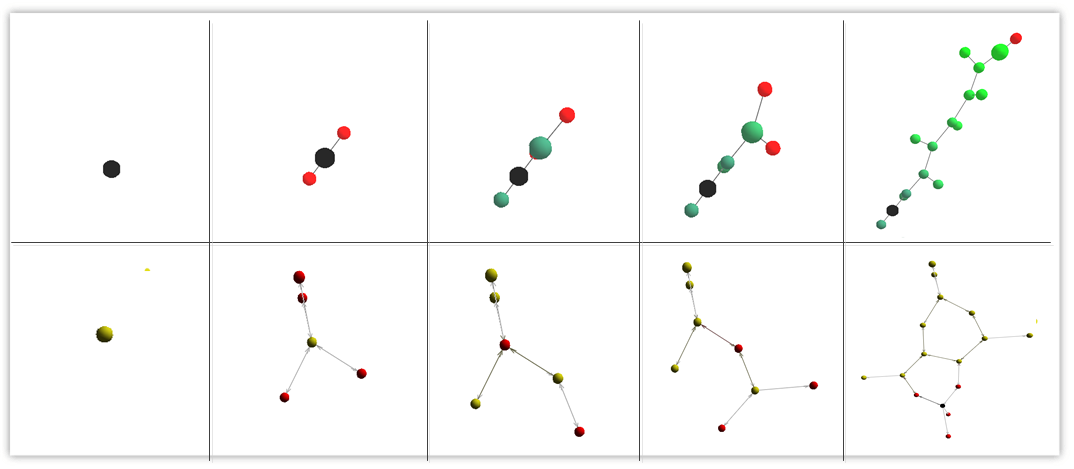
\includegraphics[width=8.5cm]{./river_prooftreegraph_step.png}
\caption{Building the proof tree and the Kripke model stepwise}
\label{fig:river_prooftreegraph_step}
%\end{figure}
%\begin{figure}[h!]
%\vspace{0.5cm}
\centering
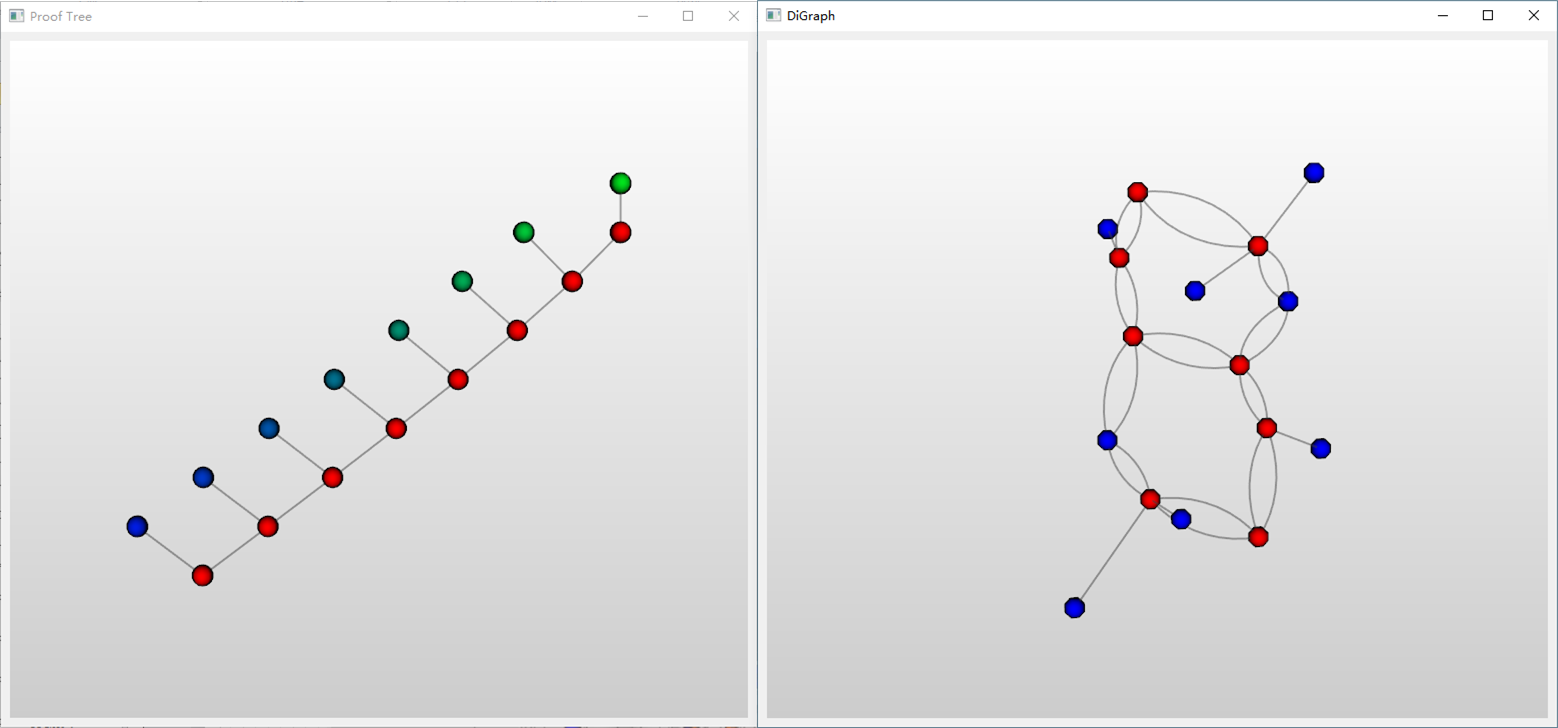
\includegraphics[width=8cm]{./river_prooftreegraph_state_highlight.png}
%\caption{A path is highlighted in the model when all the nodes in the proof tree with $EU$-formulas are highlighted}
\caption{The highlighting of all the $EU$-formulas in the proof tree (left), and a path in the model (right).}
%\vspace{-10pt}
\label{fig:river_path}
\end{figure}
%\vspace{-5pt}
 
In \textsf{SCTL}, the proof tree for formulas starting with different modalities are clearly distinguishable from each other,
the same scenario holds for the related part in the Kripke model under consideration.
For instance, the main part of a proof tree of an $EU$-formula corresponds to a finite path in the model,
testifying this proof.
While for verifying an $AG$-formula,
both the proof tree and the related part in the Kripke model may appear very complicated
(Fig. \ref{fig:ag_proof}).
In this situation, one may focus on a part of the proof tree each time,
and track the corresponding part of the state transitions (Fig. \ref{fig:ag_part_detail}).
%\vspace{-10pt}
\begin{figure}[h!]
\centering
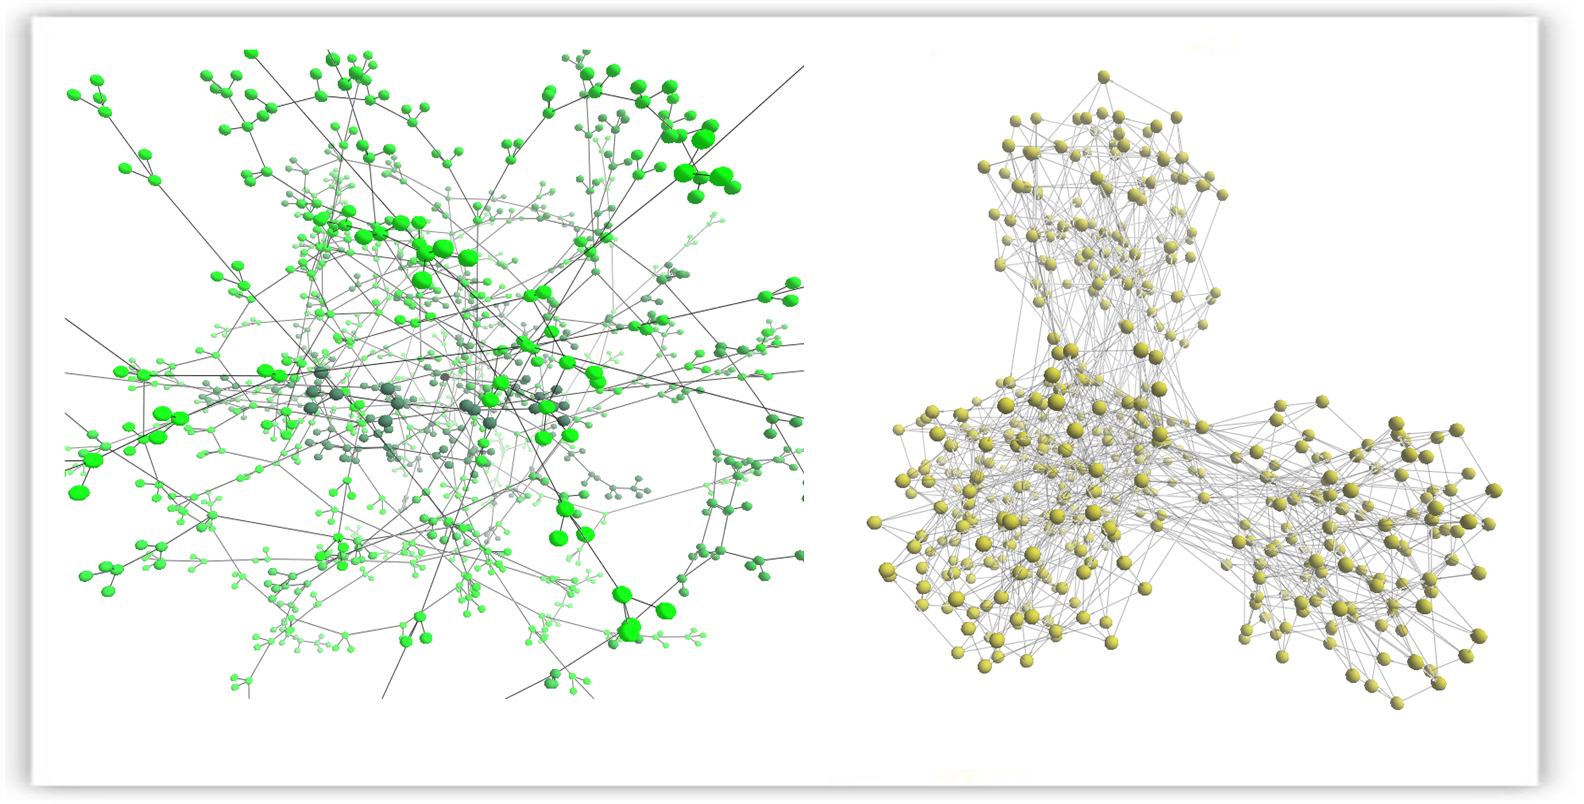
\includegraphics[width=9cm]{./ag_proof_state.png}
\caption{The proof tree (left) and the Kripke model (right) for the verification of an $AG$-formula in \textsf{SCTL}.}
\label{fig:ag_proof}
\end{figure}
\begin{figure}[h!]
%\vspace{0.5cm}
\centering
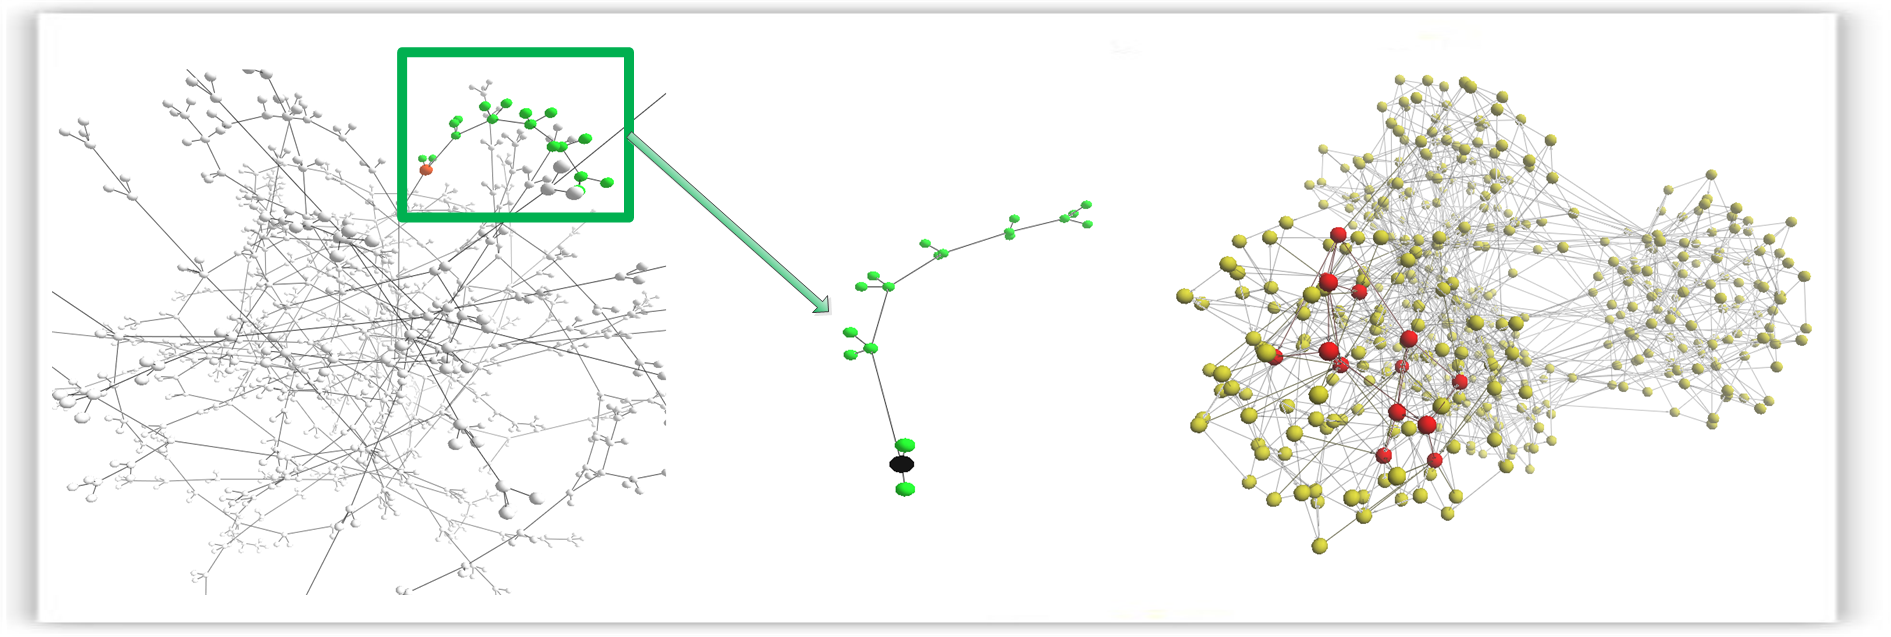
\includegraphics[width=9cm]{./ag_part_detail.png}
\caption{Focus on a subtree and highlight related state transitions}
%\vspace{-10pt}
\label{fig:ag_part_detail}
\end{figure}
 
\subsection{A Small Example of Coq}
We illustrate, by a small example, how \vmdv{} can visualize proof trees produced by Coq. In Coq, the steps of interactive proof of a formula is controlled by a proof script. Each step of the proof script introduces new proof goals based on the current proof goal. Thus, we formulate the proof tree in such a manner that each proof goal is formulated as a node, and all sub-goals of the current goal are formulated as the sub-nodes of the current node. If the current goal has no sub-goal, then the current node is a leaf node. For instance, the proof script of the formula
$${\small \forall A\; B\; C\; : Prop,\; (A\rightarrow(B\rightarrow C))\rightarrow ((A\rightarrow B)\rightarrow(A\rightarrow C))}$$
is
\begin{center}
\begin{verbatim}
Proof.
  intros A B C. intros H1 H2 H3.
  apply H1. assumption. apply H2. assumption.
Qed.
\end{verbatim}
\end{center}
There are 7 steps (the first ``assumption" comprise two steps: finish the current goal, and jump to the next goal) in this proof script. Thus, the proof tree should have 7 edges, as shown in Fig. \ref{fig:coq_example}.
 
%\vspace{-10pt}
\begin{figure}
\centering
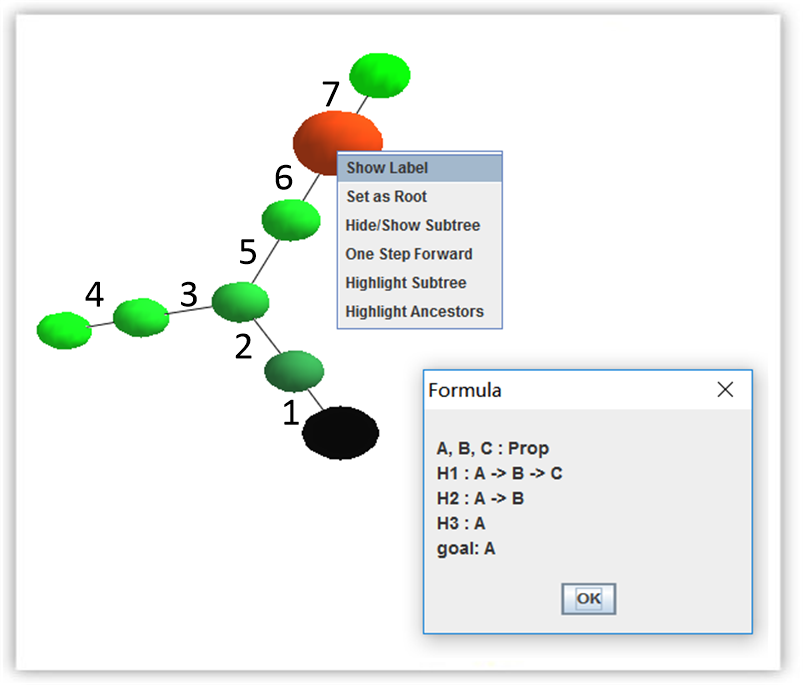
\includegraphics[width=6cm]{./coq_example.png}
\caption{Proof tree in the Coq example.}
%\vspace{-10pt}
\label{fig:coq_example}
\end{figure}
%Note that this is a naively formulation of the proof tree produced by Coq.
In order to visualize proof trees produced by Coq in \vmdv{}, one usually has two options. The first option is to build an integrated development environment (IDE) for the coq toplevel system (coqtop\footnote{\url{https://www.mankier.com/1/coqtop}}) from scratch, and let the IDE communicate with \vmdv{}. In this situation, the developer may have to handle many basic and cumbersome I/O problems of the IDE and coqtop. The second option is to build a wrapper upon existing interfaces for coqtop, such as coqide\footnote{\url{https://www.mankier.com/1/coqide}}, or Proof General\footnote{\url{https://proofgeneral.github.io/}}. These existing interfaces are usually much more flexible and easy to extend. The developer will then adapt the XML protocol specified by coqide or Proof General and translate the message into the TCP packets that are understandable by \vmdv{}, which is very straightforward. We prefer the second option, and our interface is now under development. We believe that designing such a interface would guide the interactive proof in Coq in a much more friendly way with visualization, and may be helpful in the education classes.

\section{Conclusion and Future Works}

We have proposed a visualization tool \vmdv{} for visualising (dynamically) the output of various theorem provers in 3D space, 
where an automatic layout algorithm to manage the shape of the 3D graph is used.
The focus of this paper is on the automated theorem prover \textsf{SCTLProV}, where the output is either a proof tree, or some auxiliary structure such as a Kripke model.
\vmdv{} provides us a variety of ways to observe or interact with the outputs of \textsf{SCTLProV} from a 3D perspective.


We have made our first step to the visualization analysis of proof trees produced by some automated theorem prover.
One of the main objectives for our further work is to integrate \vmdv{} with more sophisticated theorem provers such that \textsf{Coq}.
Another objective is to improve \vmdv{} so that it helps to guide proof procedures.

\section*{Acknowledgment}
The authors would like to thank the anonymous reviewers for their valuable comments.
This work was partially funded by the CAS-INRIA project VIP (GJHZ1844) and the French-Chinese project LOCALI (NSFC 61161130530 and ANR-11-IS02-00201).


%\nocite{bajaj2003interactive}
%\nocite{trac2007interactive}
%\nocite{bederson2003craft}
%brings insight into 
%\newpage
\bibliographystyle{splncs04}
\bibliography{refs}

%\appendix

%\section{The System \textsf{SCTL}}

\end{document}
